\documentclass[a4paper,12pt]{article}
\usepackage[utf8]{inputenc}

\usepackage[utf8]{inputenc}
\usepackage[T2A]{fontenc}
\usepackage[russian]{babel}
\usepackage{amsthm}
\usepackage{amsmath}
\usepackage{amssymb}
\usepackage{tikz}
\usepackage{textcomp}
\usepackage{marvosym}
\usepackage{ esint }
\setlength{\topmargin}{-0.5in}
\setlength{\textheight}{9.1in}
\setlength{\oddsidemargin}{-0.4in}
\setlength{\evensidemargin}{-0.4in}
\setlength{\textwidth}{7in}
\setlength{\parindent}{0ex}
\setlength{\parskip}{1ex}
\newcommand{\ndiv}{\hspace{-4pt}\not|\hspace{2pt}}
\usepackage{graphicx}
\usepackage{float}
\usepackage{wrapfig}
\usepackage{pgfplots}
\usepackage{caption}
\pgfplotsset{compat=1.16}
\graphicspath{ {./images/} }

\title{Лабораторная работа № 3.2.5\\Свободные и вынужденные колебания в электрическом контуре}
\author{Илья Прамский}
\date{Октябрь 2023}

\begin{document}

\maketitle
\newpage
\section*{Введение}
\textbf{Цель работы:} исследование свободных и вынужденных колебаний в
колебательном контуре.

\textbf{В работе используются:} осциллограф АКТАКОМ ADS-6142H, генератор сигналов специальной формы АКИП-3409/4, магазин сопротивления МСР-60, магазин емкости Р5025, магазин индуктивности Р567 типа МИСП, соединительная коробка с шунтирующей емкостью, соединительные одножильные и коаксиальные провода.

\subsection*{Экспериментальная установка}

Схема установки для исследования колебаний приведена на рисунке.
Колебательный контур состоит из постоянной индуктивности L с активным сопротивлением RL, переменной емкости C и сопротивления R. Картина колебаний
напряжения на емкости наблюдается на экране двухканального осциллографа. Для возбуждения затухающих колебаний используется генератор сигналов специальной
формы. Сигнал с генератора поступает через конденсатор C1 на вход колебательного контура. Данная емкость необходима чтобы выходной импеданс генератора был
много меньше импеданса колебательного контура и не влиял на процессы, проходящие в контуре.

\begin{figure}[H]
	\begin{center}
    		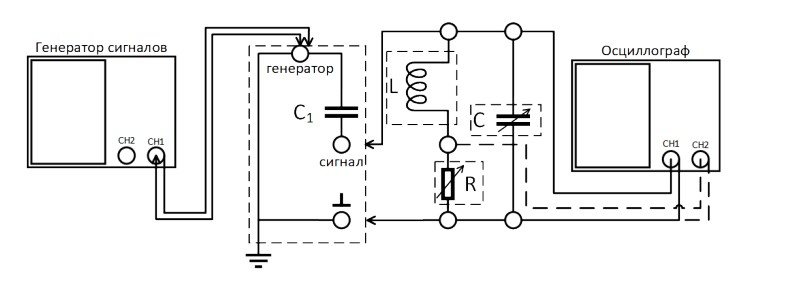
\includegraphics[width=1\textwidth]{schema.jpg}
    		\caption{Схема установки для исследования вынужденных 				колебаний}\label{fig:foobar}
    	\end{center}
\end{figure}
Установка предназначена для исследования не только возбужденных, но и свободных колебаний в электрической цепи. При изучении свободно затухающих колебаний генератор специальных сигналов на вход колебательного контура подает периодические короткие импульсы, которые заряжают конденсатор C. За время между
последовательными импульсами происходит разрядка конденсатора через резистор
и катушку индуктивности. Напряжение на конденсаторе UC поступает на вход канала 1(X) электронного осциллографа. Для наблюдения фазовой картины затухающих
колебаний на канал 2(Y) подается напряжение с резистора R (пунктирная линия на
схеме установки), которое пропорционально току I ($I \propto \frac{dU_C}{dt}$).
При изучении возбужденных колебаний на вход колебательного контура подается
синусоидальный сигнал. С помощью осциллографа возможно измерить зависимость
амплитуды возбужденных колебаний в зависимости от частоты внешнего сигнала,
из которого возможно определить добротность колебательного контура. Альтернативным способом расчета добротности контура является определение декремента
затухания по картине установления возбужденных колебаний. В этом случае генератор сигналов используется для подачи цугов синусоидальной формы.

\section*{Ход работы}
\subsection*{Измерение периодов свободных колебаний}
Для начала найдем значение емкости, которым обладает сам контур. Для этого поставим в ноль значение емкости на магазине емкостей и найдем период колебаний. В данном случае R = 0 Ом, L = 100 мГн. $T_\text{кол} = 68 $ мкс. Тогда по формуле Томсона $C_0 = \frac{T^2}{4 \cdot \pi^2 \cdot L} = 1,2$ нФ. Эту емкость в дальнейшем будем учитывать и прибавлять при расчетах. 

Теперь измерим значение периода колебаний при различных емкостях. Также посчитаем значения периодов, которые должны получится при данных параметрах системы и по этим данным построим график зависимости $T_{\text{эксп}}$ от $T_{\text{теор}}$. Учтем погрешность приборов(магазин емкостей $\delta C = 0,01$ нФ, магазин индуктивности $\delta L = 0,2 $мГн)

\begin{figure}[H]
	\begin{center}
    		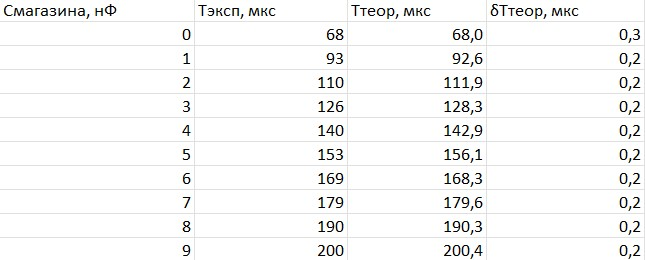
\includegraphics[width=.5\textwidth]{tabliza2.2.jpg}
    	\end{center}
\end{figure}

\begin{figure}[H]
	\begin{center}    		
    		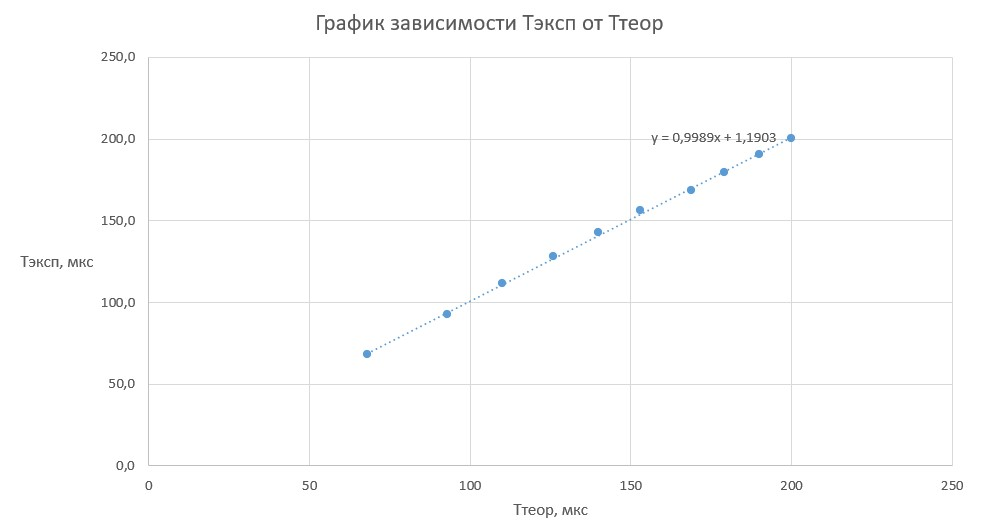
\includegraphics[width=1\textwidth]{graphik2.2.jpg}
    	\end{center}
\end{figure}
Получилось, что теоретические значения практически совпадают с экспериментальными.

\subsection*{Критическое сопротивление и декремент затухания}
Приняв L = 100 мГн, R = 0 Ом, рассчитаем значение емкости, при которой собственная частота колебаний $\nu = 6,5$ кГц. $C^\ast = 6 $ нФ. Теперь найдем $R_{cr} = 2 \cdot \sqrt{\frac{L}{C^\ast}} = 8168$ Ом.

Теперь найдем $R_{cr}$ экспериментально:для этого будем менять сопротивление до тех пор, пока колебательный режим не перейдет в апериодический. Получается $R_{cr} = 8 $ кОм. Разница между сопротивлениями возникает из-за сопротивлений индуктивности и ёмкости, а также из-за неточного определения перехода из колебательного режима в апериодический(точного перехода не видно).

Для незатухающих колебаний справедлива формула $T_0 = 2 \cdot \pi \cdot \sqrt{L \cdot C}$. Для затухающих же колебаний, период определяется несколько иным способом: $T_1 = \frac{T_0}{\sqrt{1-\frac{\gamma^2}{\omega_0^2}}}$, где $\gamma = \frac{R}{2L}$ - коэффициент затухания, $\omega_0 = \frac{1}{\sqrt{LC}}$ - собственная круговая частота контура.

Логарифмический декремент $\theta = \frac{1}{n} \cdot \ln{\frac{U_m}{U_{m+n}}} = \gamma \cdot T_1$. Получается, что
\[\theta = \gamma \cdot T_1 = \gamma \cdot \frac{T_0}{\sqrt{1-\frac{\gamma^2}{\omega_0^2}}} = \frac{\gamma \cdot 2 \cdot \pi \cdot \sqrt{L \cdot C} \cdot \omega_0}{\gamma \cdot \sqrt{\frac{\omega_0^2}{\gamma^2} - 1}} = \frac{2 \cdot \pi}{\sqrt{\frac{\omega_0^2}{\gamma^2} - 1}}\]
А так как $\frac{\omega_0^2}{\gamma^2} = \frac{4L^2}{LC \cdot R^2} = \frac{4R_{cr}^2}{R^2}$, то получается, что 
\[\theta = \frac{2 \cdot \pi}{\sqrt{\frac{R_{cr}^2}{R^2} - 1}} \]
Теперь будем менять от $0,05 \cdot R_{cr}$ до $0,25 \cdot R_{cr}$ и измерять амплитуды $U_m$ и $U_{m+n}$ разделенные целым числом периодов $n$. Получив эти данные, рассчитаем логарифмический декремент и построим график зависимости $\frac{1}{\theta^2}$ от $\frac{1}{R_\Sigma^2}$. Получилась линейная зависимость, что подтверждает справедливость полученной формулы. Зная, что в итоге должно получиться $R_{cr} = 2 \cdot \pi \cdot k$, где k- коэффициент пропорциональности, найдем $R_L = 82,07$ Ом.

\begin{figure}[H]
	\begin{center}
    		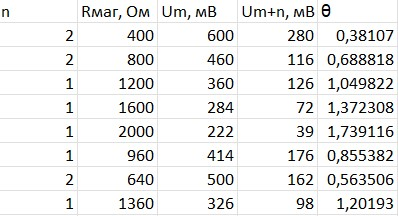
\includegraphics[width=.5\textwidth]{tabliza2.3.jpg}
    	\end{center}
\end{figure}

\begin{figure}[H]
	\begin{center}    		
    		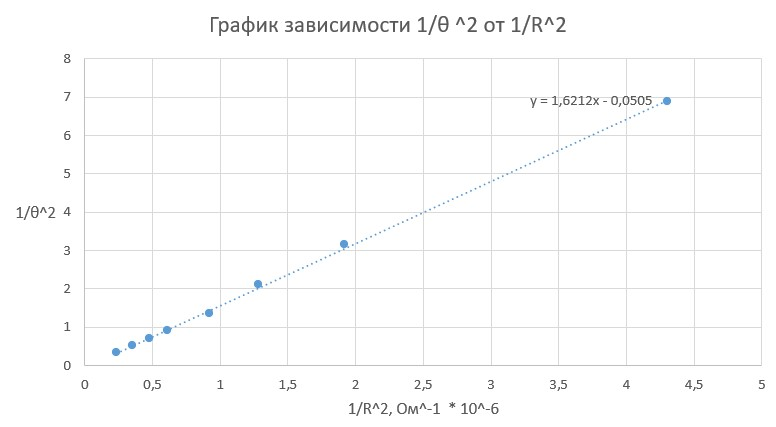
\includegraphics[width=1\textwidth]{graphik2.3.jpg}
    	\end{center}
\end{figure}

Теперь найдем добротность для двух критических значений сопротивления($Q = \frac{\pi}{\theta}$). При $R_1 = 400$ Ом, $Q_1 = 8,2 \pm 0,6$. При $R_2 = 2000$ Ом, $Q_2 = 1,8$.
\subsection*{Свободные колебания на фазовой плоскости}
Проделаем то же самое, что и в предыдущем пункте, на фазовой плоскости. Изменяя сопротивление магазина, найдем декремент, а по нему - добротность.

\begin{figure}[H]
	\begin{center}
    		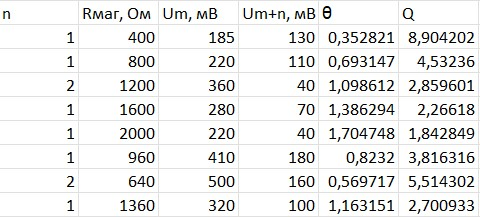
\includegraphics[width=.5\textwidth]{tabliza2.4.jpg}
    	\end{center}
\end{figure}
\subsection*{Расчет теоретического значения добротности}
Рассчитаем значение добротности для контура c $L = 100$ мГн, $C = C^\ast = 6$ нФ, $R = R_1 = 400$ Ом.
\[Q = \frac{\pi}{\theta} = \frac{\pi}{\frac{2 \cdot \pi}{\sqrt{\frac{\omega_0^2}{\gamma^2} - 1}}} = \frac{\sqrt{\frac{\omega_0^2}{\gamma^2} - 1}}{2}\]
Получается(учитывая емкость контура и сопротивление магазина индуктивностей) $Q = 7,7 \pm 0,3$.

\subsection*{Исследование резонансных кривых}
Теперь будем подавать синусоидальные сигналы, зафиксируем емкость и сопротивление $C^\ast$ и $R_1$ соответственно. Найдем резонансную частоту(при ней отсутствует разность фаз, а также наблюдается максимальная амплитуда). Получилось $\nu_{рез} = 6$ кГц, $U_{C, \text{рез}} = 17,2$ В. Теперь рассмотрим амплитуды и разности фаз вблизи резонанса, по ним построим АЧХ и ФЧХ.

$\Delta \varphi = 2 \cdot \pi \cdot \nu \cdot \Delta x$

\begin{figure}[H]
	\begin{center}
    		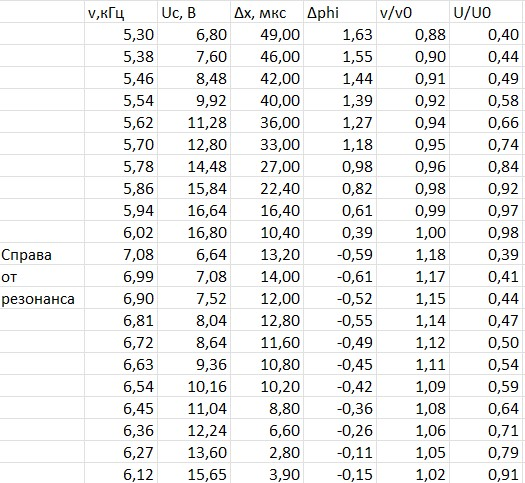
\includegraphics[width=.5\textwidth]{tabliza2.5.jpg}
    	\end{center}
\end{figure}

\begin{figure}[H]
	\begin{center}    		
    		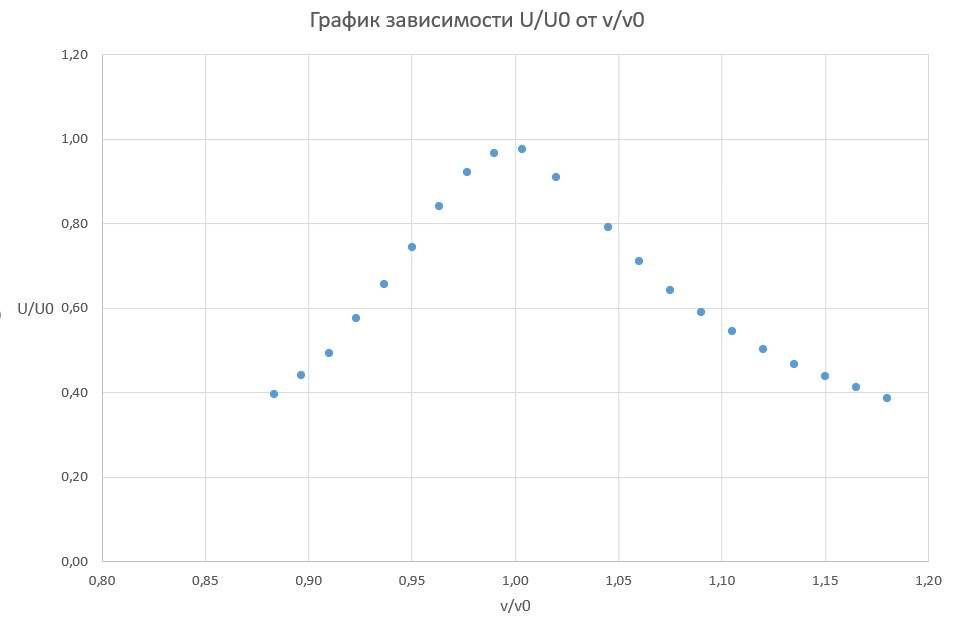
\includegraphics[width=1\textwidth]{graphik2.5.jpg}
    	\end{center}
\end{figure}

\begin{figure}[H]
	\begin{center}    		
    		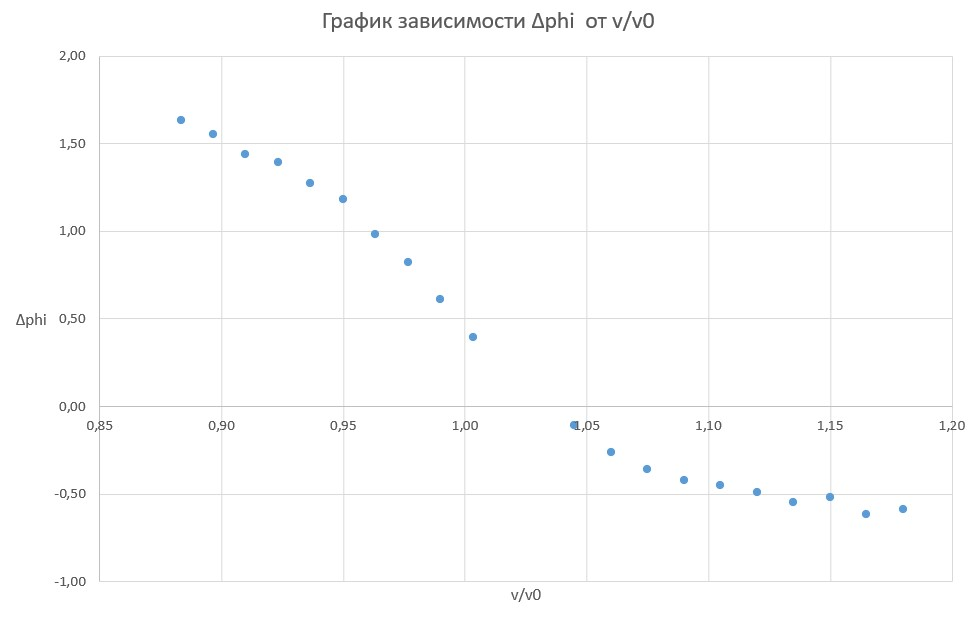
\includegraphics[width=1\textwidth]{graphik2.52.jpg}
    	\end{center}
\end{figure}

Теперь найдем добротность по АЧХ и ФЧХ.

Добротность по АЧХ $Q = \frac{\nu_0}{2 \cdot \Delta \Omega}$, где $2\Delta \Omega$ -  ширина резонансной кривой, измеренная на уровне $\frac{f(1)}{\sqrt{2}}$. Получилось $Q = 8,3 \pm 0,6$.

Добротность по ФЧХ $Q = \frac{\nu_0}{\Delta \omega}$. $\Delta \omega$ находится по алгоритму из справочного материала. Получается $Q = 10,2 \pm 0,4$.

\subsection*{Процессы установления и затухания}
Найдём логарифмический декремент затухания при нарастании и затухании вынужденных колебаний.

При нарастании
\[\theta = \frac{1}{n} \cdot \ln{\frac{U_0 - U_k}{U_0 - U_{n+k}}}\]
При затухании
\[\theta = \frac{1}{n} \cdot \ln{\frac{U_m}{U_{m+n}}}\]

\newpage
Получается

\begin{figure}[H]
	\begin{center}
    		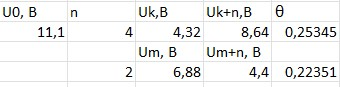
\includegraphics[width=.5\textwidth]{tabliza2.6.jpg}
    	\end{center}
\end{figure}

$Q_1 = 12,3; Q_2 = 14,1$.

\section*{Вывод}
В ходе работы были исследованы свободные и вынужденные колебания в электрическом контуре, проверена справедливость формулы периода, исследован декремент затуханий и его зависимость от суммарного сопротивления контура. Также была найдена добротность системы различными способами:теоретическим, при помощи декремента(который тоже был найден разными способами:через амплитуды, при помощи спирали на фазовом пространстве, а также при нарастании и затухании колебания), с помощью АЧХ И ФЧХ. Полученные добротности изображены на таблице. Значения находятся близко друг к другу, однако последние выбивается из них, это может быть связано с тем, что данные брались с другой установки.

\begin{figure}[H]
    		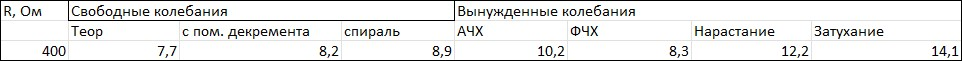
\includegraphics[width=1.05\textwidth]{tablizavivod.jpg}
\end{figure}

\end{document}

